% IEEE S&P 2027 submission format; requires IEEEtran.cls v1.8b.
\documentclass[conference,compsoc]{IEEEtran}

\usepackage[T1]{fontenc}
\usepackage[utf8]{inputenc}
\usepackage{booktabs}
\usepackage{tabularx}
\usepackage{array}
\usepackage{graphicx}
\usepackage{amsmath}
\usepackage[dvipsnames,table]{xcolor}
\usepackage{tikz}
\usetikzlibrary{arrows.meta,positioning,fit,calc,matrix,shapes.geometric}
\usepackage[hyphens]{url}
\usepackage{hyperref}

\hypersetup{hidelinks,pdfauthor={}}
\newcommand{\scope}{\textsc{Scope}}
\newcommand{\NRR}{\textsc{nr-r}}
\newcommand{\NRA}{\textsc{nr-a}}
\newcommand{\NRV}{\textsc{nr-v}}
\newcommand{\NA}{\textsc{na}}
\newcommand{\evidenceStrong}{\cellcolor{ForestGreen!22}Strong}
\newcommand{\evidenceLimited}{\cellcolor{Goldenrod!24}Limited}
\newcommand{\evidenceNone}{\cellcolor{Gray!18}No verified direct evidence}
\newcolumntype{Y}{>{\raggedright\arraybackslash}X}
% Additive finite-candidate reconciliation; historical snapshots retained.
\newcommand{\SnapshotN}{60}
\newcommand{\SnapshotCore}{43}
\newcommand{\SnapshotA}{15}
\newcommand{\SnapshotB}{28}
\newcommand{\SnapshotAdjacent}{17}
\newcommand{\FinalN}{82}
\newcommand{\FinalCore}{58}
\newcommand{\FinalA}{20}
\newcommand{\FinalB}{38}
\newcommand{\FinalAdjacent}{24}


\title{SoK: When Do LLM Side-Channel Defenses Protect Agent Workflows?}
\author{}
% Original 60-family snapshot: October 8; bounded retrieval update: October 21.
% New controlled placement study has a separate frozen protocol and raw receipts.

\begin{document}
\maketitle

\begin{abstract}
When does protecting an LLM service protect an agent workflow? We systematize defense evidence by binding each result to its receiver, execution boundary and evaluated mechanism. Three checks follow: locate the final target-bearing emitter, validate cover at execution, and match adaptation and cost to the protected condition. Source-backed cases and a 33-result comparison audit identify when measurements can be reused. Two controlled experiments test the first two checks using new Luna outputs and plans. Upstream padding reduces size-based inference to chance at its own link, while a new terminal emitter remains distinguishable; final-link padding removes this size feature. Discarded, isolated and read-only cover preserve all 24 task states, whereas live writes leave nine complete successes. The evidence map combines the original collection with a bounded retrieval update. The contribution is actionable conditions for reusing defense results, supported by explicit comparisons, positive reuse cases and inspectable controlled interventions.
\end{abstract}

\section{Introduction}\label{sec:introduction}
Encryption conceals content but need not conceal execution. LLM services produce token streams, cache hit/miss timing and shared-resource activity; agents add destinations, tool exchanges and website actions. A receiving website, a passive network observer and an active API client see different projections \cite{weiss2024prompt,promptpeek2025,earlybird2025,agentprint2025,uitraces2026,jeong2026wra}. The practical question is which deployment decision a favorable defense result actually supports.

A designer choosing padding, cover traffic or action humanization faces a concrete difficulty: similar defense labels refer to different protected objects. NetEcho studies downstream re-emission, the Web and Research Agents (WRA) study uses concurrent decoy requests for privacy, Dangol measures transport cover, and the Agent Humanization Benchmark (AHB) measures executed mobile humanization \cite{netecho2025,jeong2026wra,dangol2026workflow,zhu2026turing}. A lower inference score, preserved task success and a small component overhead are useful findings, but they answer different deployment questions. Reading them as one defense ranking loses the conditions that make each result useful.

\paragraph{Central insight: follow both the trace and the action}
Protecting a communication trace and preserving an agent's task are separate obligations. A downstream frontend can emit a new target-bearing trace after upstream protection; a dummy that enters tool or GUI execution can alter the task itself. The distinction changes the appropriate evaluation. A new emitter calls for final-hop capture; surviving features call for an adapted predictor; executed cover calls for objective task and policy checks. These tests address different failure mechanisms and cannot substitute for one another.

We turn these source findings into three worked deployment decisions (Section~\ref{sec:discussion}): choose the final interface to protect, decide whether cover may execute, and select an applicable adaptation result and cost. Each case states what can be adopted from existing evidence and what condition would permit reuse elsewhere. For example, verified discard before semantic dispatch excludes direct fake-action state changes while leaving resource and delay effects to be checked. The same tested receiving view supports its local adaptation result; a different view requires a capture bridge. This cross-paper mapping is the contribution: the original papers establish the component phenomena, and the synthesis makes their consequences usable for system design.

\paragraph{Contributions and use}
The paper contributes (1) three source-backed deployment decisions with explicit conditions for reusing a result; (2) an eight-type defense map and a quantitative audit of result comparability and reporting; (3) two controlled placement experiments using new Luna responses and tool plans; and (4) source-linked records that make these judgments reconstructible. A completed, bounded retrieval update extends the original 60-family snapshot to \FinalN{} families (Section~\ref{sec:methodology}). The collection supplies context and counterconditions; source measurements and the controlled interventions supply each case's evidence. Privileged diagnostics, attribution and human--agent distinction are distinguished from confidentiality leakage.

Figure~\ref{fig:system-model} separates the trace and action paths; Figure~\ref{fig:defense-decision} gives the three-check procedure. Section~\ref{sec:discussion} works through its cases, Section~\ref{sec:defenses} audits the evidence, and Section~\ref{sec:controlled-placement} tests receiver and execution placement. The checklist in Section~\ref{sec:agenda} translates the cases into reporting practice. Public-trace reanalysis, failed runs and the negative checklist comparison remain in the Supplementary Evidence.

\begin{figure*}[t]
\centering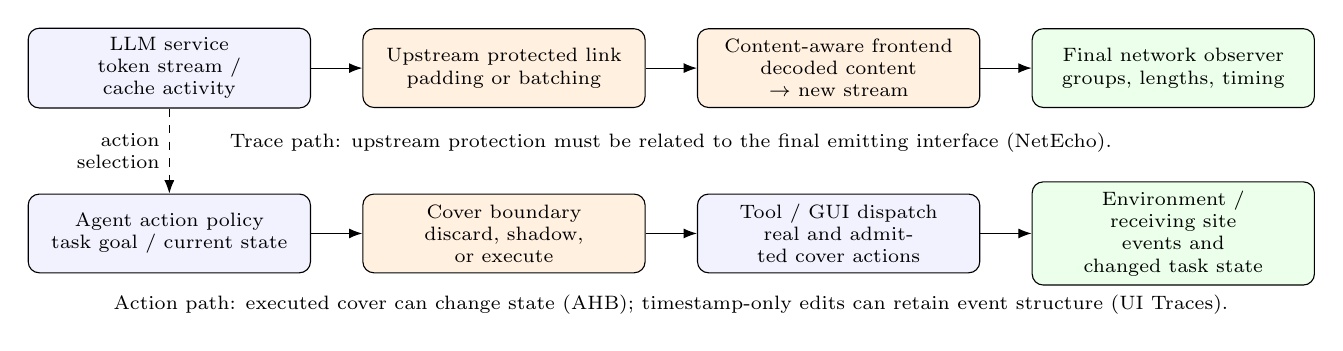
\begin{tikzpicture}[font=\scriptsize,>=Latex,
box/.style={draw,rounded corners,align=center,text width=3.35cm,minimum height=10mm,fill=blue!5},
boundary/.style={box,fill=orange!12},
observer/.style={box,fill=green!8}]
\node[box] (llm) at (0,0) {LLM service\\token stream / cache activity};
\node[boundary] (api) at (4.25,0) {Upstream protected link\\padding or batching};
\node[boundary] (front) at (8.5,0) {Content-aware frontend\\decoded content $\rightarrow$ new stream};
\node[observer] (net) at (12.75,0) {Final network observer\\groups, lengths, timing};
\draw[->] (llm)--(api);
\draw[->] (api)--(front);
\draw[->] (front)--(net);
\node[box] (policy) at (0,-2.1) {Agent action policy\\task goal / current state};
\node[boundary] (cover) at (4.25,-2.1) {Cover boundary\\discard, shadow, or execute};
\node[box] (dispatch) at (8.5,-2.1) {Tool / GUI dispatch\\real and admitted cover actions};
\node[observer] (state) at (12.75,-2.1) {Environment / receiving site\\events and changed task state};
\draw[->] (policy)--(cover);
\draw[->] (cover)--(dispatch);
\draw[->] (dispatch)--(state);
\draw[->,dashed] (llm.south)--node[left,align=right]{action\\selection}(policy.north);
\node[font=\scriptsize,align=center] at (6.37,-.95)
{Trace path: upstream protection must be related to the final emitting interface (NetEcho).};
\node[font=\scriptsize,align=center] at (6.37,-3.0)
{Action path: executed cover can change state (AHB); timestamp-only edits can retain event structure (UI Traces).};
\end{tikzpicture}

\caption{Two paths that a deployment judgment must follow. The top path distinguishes an upstream protected link from a new downstream emitter; the bottom distinguishes communication cover from actions admitted to execution. The diagram organizes source mechanisms, not one jointly evaluated system.}
\label{fig:system-model}
\end{figure*}

\begin{figure*}[t]
\centering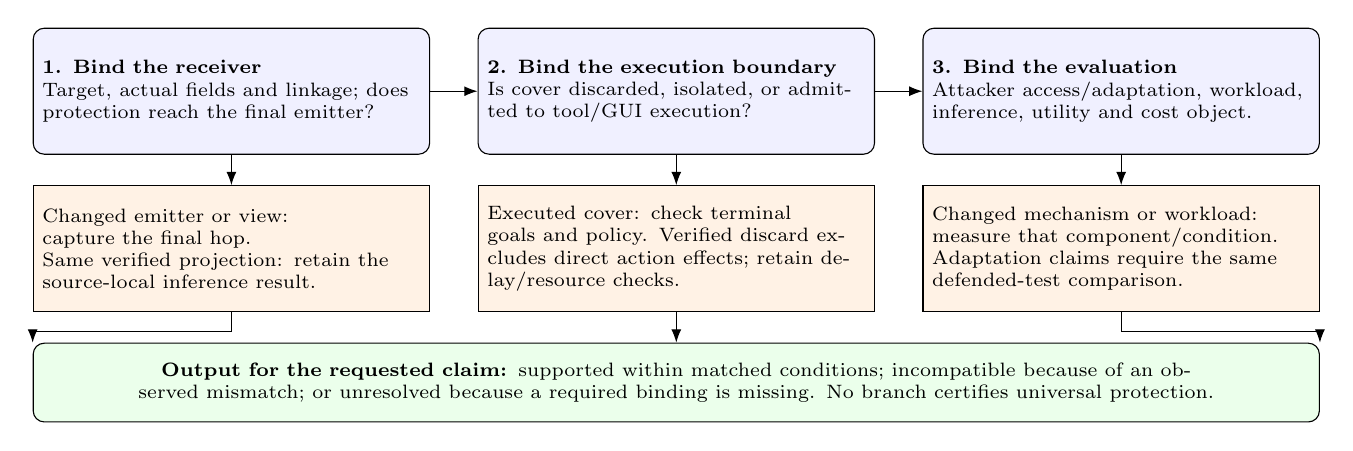
\begin{tikzpicture}[font=\scriptsize,>=Latex,
check/.style={draw,rounded corners,fill=blue!6,align=left,text width=4.8cm,minimum height=16mm},
test/.style={draw,fill=orange!10,align=left,text width=4.8cm,minimum height=16mm}]
\node[check] (receiver) at (0,0) {\textbf{1. Bind the receiver}\\Target, actual fields and linkage; does protection reach the final emitter?};
\node[check] (action) at (5.65,0) {\textbf{2. Bind the execution boundary}\\Is cover discarded, isolated, or admitted to tool/GUI execution?};
\node[check] (effect) at (11.3,0) {\textbf{3. Bind the evaluation}\\Attacker access/adaptation, workload, inference, utility and cost object.};
\draw[->] (receiver)--(action);
\draw[->] (action)--(effect);
\node[test] (rtest) at (0,-2.0) {Changed emitter or view:\\capture the final hop.\\Same verified projection: retain the source-local inference result.};
\node[test] (atest) at (5.65,-2.0) {Executed cover: check terminal goals and policy. Verified discard excludes direct action effects; retain delay/resource checks.};
\node[test] (etest) at (11.3,-2.0) {Changed mechanism or workload:\\measure that component/condition.\\Adaptation claims require the same defended-test comparison.};
\draw[->] (receiver)--(rtest);
\draw[->] (action)--(atest);
\draw[->] (effect)--(etest);
\node[draw,rounded corners,fill=green!8,align=center,text width=16.1cm,minimum height=10mm] (out) at (5.65,-3.7)
{\textbf{Output for the requested claim:} supported within matched conditions; incompatible because of an observed mismatch; or unresolved because a required binding is missing. No branch certifies universal protection.};
\draw[->] (rtest.south)--++(0,-.25)-|(out.north west);
\draw[->] (atest)--(out);
\draw[->] (etest.south)--++(0,-.25)-|(out.north east);
\end{tikzpicture}

\caption{Three checks for applying a reported defense result. Each identifies a positive reuse condition and the evidence needed when the deployment changes.}
\label{fig:defense-decision}
\end{figure*}

\section{Scope and Review Method}\label{sec:methodology}\label{sec:background}
\subsection{Questions and eligibility}
We ask which hidden targets and observables appear (RQ1), how signal origin relates to receiver permission (RQ2), what establishes feasibility and transfer (RQ3), and which intervention addresses which observable at what cost (RQ4). An agent selects and executes actions using an LLM, tools, memory or orchestration; inherited serving and hardware channels need not be agent-specific.

Core eligibility requires (C1) LLM/agent execution, (C2) a hidden target, (C3) an execution-dependent auxiliary observable rather than ordinary output semantics alone, (C4) specified observation permissions, and (C5) an empirical inference evaluation. A controlled synthetic-state inference can satisfy C5; a proposed mechanism or timing gap alone cannot. Mixed papers qualify through an identifiable component. Table~\ref{tab:boundary-rules} supplies the decision rules.
\begin{table}[t]\centering\footnotesize
\caption{Observable-based eligibility. A hidden target alone does not make a semantic attack a side channel.}\label{tab:boundary-rules}
\begin{tabularx}{\columnwidth}{@{}p{.39\columnwidth}Y@{}}\toprule
Observed input & Decision and required distinction\\\midrule
Length, timing, cache response & Core when measured execution dependence supports hidden-target inference.\\
Own-site actions & Core attribution with site permission; no automatic access to other sites or private tool logs.\\
Reply states the secret & Direct disclosure; adjacent, not auxiliary-channel evidence.\\
Reply style/content identifies a user & Adjacent unless a separately evaluated auxiliary mechanism is established. WildAuth stays a mixed-view comparator.\\
Output-filter membership oracle & Can be core: the filter's execution, not ordinary semantic output inference, mediates the signal.\\
Privileged loop/fault logs & Separate diagnostic component when C1--C5 hold; does not increase confidentiality evidence.\\\bottomrule
\end{tabularx}\end{table}


The final coded collection contains \FinalN{} version-bound families, with retrieval updated through October 21, 2026: \FinalCore{} core (\FinalA{} workflow-origin, \FinalB{} inherited-runtime/application) and \FinalAdjacent{} adjacent. Five core components concern authorized diagnostics. Other targets include content/property inference, provenance attribution and human/agent distinction; hiddenness alone establishes no confidentiality violation. Families are deduplicated studies; result records distinguish conditions within a study. The original October 8 snapshot (60 families, 43 core) is retained separately: its 33-result/66-field audit remains a named subset, not a census of the enlarged collection.

The auxiliary-only rule is applied consistently. Coding fingerprints and WildAuth remain adjacent because their evaluated views mix semantic and interaction features; feature importance is not a separately evaluated auxiliary-only attack \cite{ghaleb2026codingfingerprint,wang2026dialogue}. Metric-only fault localization qualifies as a diagnostic component despite operator authorization \cite{scheinert2026rca}. ZeroPrint's response differences, endpoint-content fingerprints and StepFinder's mixed view remain adjacent \cite{shao2026zeroprint,leshin2026endpoint,zhu2026stepfinder}.

\subsection{Purposive sampling and citation tracing}
This SoK uses purposive, mechanism-oriented sampling supplemented by fixed one-hop backward and forward citation tracing. It synthesizes decision-relevant evidence rather than estimating literature-wide prevalence. Acquisition combines native IEEE Xplore/ACM Digital Library exports, targeted discovery of preprints/proceedings with exact-title/DOI primary-source lookup, and tracing from 40 fixed seeds. Targeted searches covered arXiv and primary USENIX, NDSS and PMLR records. Appendix~\ref{app:search} gives executable native queries; Supplement S1 retains their exports and targeted query logs. All 2,237 returned backward reference occurrences and 24 distinct forward works were screened; forward lookup resolved 38 of 40 seeds. Versions are merged only with identity evidence.

We distinguish the acquired candidate frames from the coded collection. The prepared metadata frame contains 4,753 unique IDs with a recorded exclusion, referral or unresolved disposition. A bounded source reconciliation accounts for 109 overlapping decision rows in four nominated frames (57 follow-ups, six proposals, 22 backward candidates and 24 forward records). The map retains source-unavailable outcomes; it is not 109 independent full readings. At the source-search endpoint, unavailable full texts and unestablished empirical components are not admitted to the present core analysis. Unbound defense quantities are excluded from matched comparisons without removing their qualifying attack families.

The saved native exports contain only 1/24 (IEEE) and 0/24 (ACM) fixed known papers, demonstrating that they are inadequate as the sole acquisition route. We therefore completed an additional finite search frame: four Semantic Scholar bulk queries and two native arXiv searches returned 615 occurrences, deduplicated to 565 records. Every record has a reasoned route, source fragment and receipt; 49 received source-scoped examination. Fifteen new core and seven selected adjacent families were incorporated. Sixteen missing-abstract records and one unavailable primary full text remain material requests, not exclusions or core admissions. Supplement S10 gives the executable queries, completed frame, failed accesses and full disposition counts.

The update recovers 17/24 fixed known papers and 25/60 original families. Because indexing and field eligibility are not established for every non-return, these are query-recovery counts, not calibrated recall. The incomplete broad IEEE/ACM frames remain historical acquisition gaps, separate from the completed 565-record frame. An exclusion check covered all 177 high-risk exclusions and 27 reason-stratified samples (seed 20261021), rerouting four records: one new core, one existing-family alias and two adjacent contexts. This same-workflow check measures observed corrections, not an independent false-negative rate. Countercondition searches and source-deletion analysis test the specific synthesis without claiming exhaustive coverage.

\subsection{Coding, adjudication and reproducibility}
The extraction dictionary specifies receiver permissions, auxiliary versus semantic observations, result splitting, execution mode, utility/cost object and source/run binding. Source-scoped \NRR{}, unavailable \NRA{} and unverified \NRV{} remain distinct from replication. Code inspection can establish implementation behavior without authenticating the historical run.

One coding workflow used AI assistance in screening, extraction, source rechecks and writing. Disagreements were resolved against source text and recorded with locators. Supplement S1 retains the 23-case blinded AI exercise (17/21 determinate agreement), 332-dispute readbacks and exclusion audits. They are AI-assisted checks, not independent human coding or a human agreement estimate. The result records and conclusion dependencies expose the interpretations for direct inspection.

The Supplementary Evidence supplies the \FinalN{}-family merged index and the original 60-family index. All 43 original core families have a scoped intervention disposition; the update separately extracts observation, target, evaluation, mitigation, utility and cost for each of its 15 core additions. The original 33 result records, 66 utility/cost positions and pairwise/checklist audit retain their original denominator. Section~\ref{sec:scope} gives a complete record-to-judgment example. Supplements S6/S10 test source deletion and collection expansion; S8 supplies the original comparison audit. All records retain source versions, locators, unknown fields and claim dependencies.

\section{Result Records and Comparison Rules}\label{sec:scope}
The unit of comparison is one evaluated condition, rather than a paper or a headline score. A result record binds a source version and locator to its target, receiver, intervention, attacker procedure, workload and outcomes (Table~\ref{tab:result-record}). A family can contribute several records when it reports different execution modes, protected views or cost components. This is why a valid result can answer one deployment question while leaving another unresolved.
\begin{table}[t]\centering\footnotesize
\caption{A single result record. Only fields relevant to the requested comparison must align; unavailable required fields remain unresolved.}\label{tab:result-record}
\begin{tabularx}{\columnwidth}{@{}p{.24\columnwidth}Y@{}}\toprule
Record field & Required meaning\\\midrule
Source & Family/result ID, version, source locator, reading scope and hash.\\
Target & Hidden property, inference goal and protection relation: confidentiality, attribution, human/agent distinction or authorized diagnosis.\\
Receiver & Actual permission and released representation, including session/document linkage and any auxiliary inputs.\\
Intervention & Where protection ends; whether edits affect stored traces, transmission or executed actions.\\
Attacker & Fit/calibration condition, test population, training access and adaptation budget.\\
Workload & Task, system, topology/hardware and grouping/holdout.\\
Outcomes & Inference metric/denominator; objective or proxy utility; applicable cost object; uncertainty and field states.\\\bottomrule
\end{tabularx}\end{table}


\paragraph{Fields, not a competing framework}
The mnemonic \scope{} expands to Secret/target, Channel, Observer, Pipeline and Exploitation goal. It is a record-field schema. Source/evaluation columns, historically called the Evidence Plane, supply provenance and experimental conditions for the same record. Generating layers span hardware, serving, transport, application/API, orchestration, tools/MCP, environment and multi-agent communication; they can differ from the receiving layer. Permission, activity, calibration access and protection relation remain separate fields. Appendix~\ref{app:notation} provides the compact key used by the detailed tables.

\paragraph{Three comparison outcomes}
A \emph{compatible} comparison has evidence for the fields needed by the requested inference. An \emph{incompatible} comparison has a positively established mismatch, such as token payload versus wire bytes or stored timestamps versus executed actions. An \emph{unresolved} comparison lacks a necessary binding or transfer test. Only the affected inference is withheld: an unreported task endpoint does not invalidate a measured bandwidth cost. Table~\ref{tab:comparison-contracts} applies these outcomes to descriptive comparison, paired effects and deployment transfer.
\begin{table}[t]\centering\footnotesize
\caption{Comparison rules. A known mismatch and a missing binding have different consequences.}\label{tab:comparison-contracts}
\begin{tabularx}{\columnwidth}{@{}p{.28\columnwidth}Y@{}}\toprule
Requirement & Condition and resulting license\\\midrule
Descriptive comparison & Align target, receiver permission, metric meaning and cost object. Different systems may be described together; token payload and wire bytes cannot be ranked as the same cost.\\
Paired effect & Compare the same defended test units and outcome. A known test-unit mismatch makes that subtraction incompatible; an unverified fit binding leaves the effect unresolved.\\
Deployment transfer & Establish a bridge for the changed receiver, intervention, workload, topology or hardware. A demonstrated violation blocks the proposed transfer; an untested bridge leaves it unresolved. Permit only the range and endpoints actually covered.\\\bottomrule
\end{tabularx}\end{table}


\paragraph{Missingness and adaptation}
\NRR{} records a quantity unreported within the inspected source scope; \NRA{} records unavailable material; \NRV{} records an unverified field, version or run binding; \NA{} records inapplicability. A missing field gives an unresolved judgment, not an observed mismatch. Fitting on protected data (D1) and comparing clean- versus protected-trained procedures on the same defended test population (D2) are separate entries in the attacker column. Neither alone establishes that the observer can obtain the labeled data or afford the fitting budget.

\paragraph{A complete traceable example}
Table~\ref{tab:result-lineage} connects a family, a result, the inspected source and the deployment judgment. The same identifiers join the supplied family index, result ledger and claim links; full source hashes and reading scopes remain in the companion evidence package.
\begin{table}[t]\centering\footnotesize
\caption{Filled record and its licensed judgment. Values are source-reported; no cross-mode effect is computed.}\label{tab:result-lineage}
\begin{tabularx}{\columnwidth}{@{}p{.24\columnwidth}Y@{}}\toprule
Join key / field & Entry\\\midrule
Family / result & \texttt{dangol2026workflow} / \texttt{DANGOL-livebinding}.\\
Version / locator & arXiv:2606.07150v3, \S9.7, live-protocol paragraph after Table~5 \cite{dangol2026workflow}.\\
Target / view & Workflow classification from live Oblivious HTTP (OHTTP)/Agent-to-Agent (A2A) traffic; not GUI-state observation.\\
Intervention & Live fixed-rate cover with fresh per-session identifiers, distinct from transformed stored captures.\\
Workload / testbed & Workflow classes with client, relay, gateway and agent co-located on one loopback host.\\
Outcome / cost & Accuracy 0.30; about 13$\times$ bytes and 11$\times$ latency in that condition.\\
Unresolved fields & Objective terminal task utility \NRR{}; precise paired live-refit comparison \NRV{}.\\
Licensed judgment & These costs describe this live protocol condition. They neither price dummy GUI actions nor prove task preservation. A matched objective endpoint is needed for the latter.\\\bottomrule
\end{tabularx}\end{table}


\paragraph{Positioning the schema}
The contribution is the source-linked decisions produced from these fields, not an advantage of the mnemonic over a checklist. A retained 512-root constructed-task comparison gives 32.16\% joint correctness for receiver traversal versus 40.63\% for a flat checklist and 45.12--45.31\% for a structured checklist. We therefore use the field schema for indexing only. Supplement S7 preserves the original endpoint, negative comparison and missing-score treatment.

\section{Corpus Map and Nearest Prior Work}\label{sec:corpus-map}
\subsection{Origins and receiving projections}
Runtime/application-inherited signals arise from inference, serving and application mechanisms; agent-native signals arise from orchestration, tools, browser actions and multi-agent execution. Origin is not receiver location. Supplement S2 maps all source-coded origins and the load-bearing source--receiver--intervention paths, distinguishing diagnostic components from confidentiality claims. These maps locate relevant evidence; the three cases make the deployment judgments.

\paragraph{Inherited channels}
Weiss reconstructs candidate text from encrypted length sequences; NetEcho's semantic information recovery is not exact-text recovery \cite{weiss2024prompt,netecho2025}. Whisper Leak classifies topics from traffic, while Time Will Tell uses aggregate completion time \cite{whisperleak2025,timewilltell2024}. Different targets and metrics prevent treating their percentages as attack strength. Chosen-request cache attacks use shared-state timing oracles; local CPU-cache and GPU interference attacks require different permissions \cite{promptpeek2025,earlybird2025,inputsnatch2024,spliceleak2026,spillbeans2025,gu2026behindbars}. LeakyLMs' architecture branch requires same-GPU-class calibration; KVGov separates hardware timing, simulated inference/defense and analytic controls \cite{majidi2026leakylms,addagada2026kvgov}.

\paragraph{Workflow channels and target relations}
AgentPrint, the Web and Research Agents (WRA) study, and the traffic benchmark infer identities, activities or traits through flow/destination structure. UI Traces and FP-Agent use own-site behavior or browser attributes \cite{agentprint2025,jeong2026wra,pouryousef2026traffic,uitraces2026,wang2026fpagent}. URL and domain views are distinct; passive encrypted observation does not reveal endpoint method semantics. AgentTell's probe site, PlanTwin's planner and SICC's authorized recipient occupy still different projections \cite{shahriar2026agenttell,yu2026plantwin,xu2026sicc}.

The \FinalCore{} core families include 53 non-diagnostic components and five privileged diagnostics: ClawGuard, cycle detection, LumiMAS, LLM-serving fault localization and MIRAGE. Fault localization uses 120 controlled fault injections and supplied onset times; MIRAGE uses internal residual-stream hooks. Neither is a low-permission privacy observer \cite{scheinert2026rca,revankar2026mirage}. Model/human attribution is not by itself a confidentiality violation. Coding fingerprints, WildAuth, SymDiag, ZeroPrint, endpoint fingerprints and StepFinder are adjacent semantic-boundary comparisons. AgentDAM is a background data-minimization benchmark, not auxiliary inference \cite{ghaleb2026codingfingerprint,wang2026dialogue,cui2026symdiag,agentdam2025}. The target-relation ledger records these differences without converting every hidden property into a protected secret.

The update adds active tool-policy audits and structural campaign linkage \cite{fayolle2026webagents,wang2026agentprov,wang2026lidar,park2026crosscampaign}, routing histories \cite{chen2026routingmetadata}, and distinct physical, sparsity and page-migration observers \cite{hadad2026shape,alhalawani2026physicaledge,chen2026sparleak,jo2026sparseety,nazaraliyev2026page404}. SplitDecoy qualifies through zero/nonzero gradient-row support, not tensor-content inversion \cite{politis2026splitdecoy}. The latter boundary keeps visual-token and gradient-value reconstruction adjacent \cite{zhou2026visionencoder,politis2026gradients}. These additions expand the observer map rather than supply interchangeable private-goal attacks.

\subsection{What earlier systematizations already establish}
Prior systematizations establish cross-layer composition and the scope of inference-to-agent transfer. Banerjee et al. organize compound-system attacks by cross-layer mechanisms and MITRE threat models; Forough et al. v2 distinguish transferable inference protection from memory/action/coordination requirements under confidential computing \cite{banerjee2024compound,forough2026secrets}. Kotevska et al. explicitly bind asset, observer, channel, permitted disclosure, guarantee and evidence in a six-element contract and claim register; their composition conditions are stated as conjectures \cite[Sections III--IV]{kotevska2026privacyfoundations}. Thus neither an observer-conditioned tuple nor a generic composition warning is new here. Our increment is the source-bound result inventory, explicit pairwise reuse decisions, the execution-state criterion for cover, and controlled tests of receiving/execution placement.

Debenedetti's auxiliary-component privacy channel, also cited by Banerjee, supplies a shared composition precursor. Our increment is the result-level decision: which existing measurement licenses a proposed deployment, and which bridge would make another result applicable? NetEcho motivates final-hop measurement after upstream protection; WRA/AHB distinguish a privacy-oriented reason to execute decoys from their possible task-state effects. Likewise, Forough distinguishes a trusted execution environment (TEE) boundary from side-channel resistance; the Early Bird/KVGov comparison makes the consequence concrete through matching primitives, calibrated oracles and measured cost components. Section~\ref{sec:discussion} turns these distinctions into permitted uses of the existing evidence.

Classical website-fingerprinting defenses establish traffic--cost trade-offs: Tamaraw studies shaping and bandwidth bounds, WTF-PAD uses adaptive padding, FRONT randomizes padding near the trace front, and Walkie-Talkie combines half-duplex communication with burst molding \cite{cai2014systematic,juarez2016wtfpad,gong2020front,wang2017walkietalkie}. The agent-specific comparison follows what happens after protection terminates: a content-aware frontend can emit another signal, and a cover action can enter task execution. Lahjouji--Colaco address agent data surfaces and governance \cite{lahjouji2026datacentric}; Kim and Horv\'ath et al. supply complementary agent-security and physical-channel maps \cite{kim2026agenticsok,horvath2024physical}. Supplement S2 gives the full prior-work comparison. Our added artifact is a result-to-decision map, not another claim to have discovered cross-layer composition.

\section{Three Deployment Decisions}\label{sec:discussion}
The three checks in Figure~\ref{fig:defense-decision} answer concrete design decisions. Table~\ref{tab:synthesis-decisions} collects the resulting permissions and boundaries so that each case can focus on what changes in the deployment judgment.

\subsection{Case 1: choose the final interface to protect}
\paragraph{Decision and relevant evidence}
An application designer must decide whether upstream API padding or batching also protects the user-facing connection after a content-aware frontend. NetEcho identifies the relevant receiving path: Trace A is token counts per group; Trace B estimates token/group character lengths. A downstream application can consume decoded upstream content or stream state and emit finer-grained network observations \cite{netecho2025}. Captured deployment configurations and locally implemented active-defense settings are distinct source results. Neither exact text nor original generation timestamps are automatically recovered.

\paragraph{What changes after binding}
An upstream padded link answers a different question from protection of the final emitter. NetEcho's authors already establish re-emission in their systems. The joint synthesis specifies the next measurement: capture the last target-bearing interface rather than merely refit on the upstream trace. UI Traces offers a contrasting case: modifying stored timestamps preserves action types and order, so the first question is which surviving features predict identity \cite{uitraces2026}. Refitting that view cannot certify a different downstream one.

SplitDecoy supplies an independent receiving-path countercondition: decoys obscure a forward split-model view, yet zero/nonzero support in the returned gradient identifies the real rows on every tested frame across nine seeds \cite[Sections 5.1--5.3]{politis2026splitdecoy}. Its authors already identify this defect. The synthesis places it beside NetEcho: inspect every target-bearing outgoing path, not only the interface on which protection was evaluated. Section~\ref{sec:controlled-placement} independently demonstrates loss and restoration of size equalization at a new terminal emitter.

\paragraph{When transfer is permitted}
The source-local inference result applies when the receiver obtains the tested projection under its evaluated population and condition. A stronger information-theoretic permission has a precise form.

\noindent\textbf{Proposition 1 (protected-only postprocessing).}
Let $S$ be the hidden target, $Z$ the complete protected representation and $Y$ the downstream observation. If $S\to Z\to Y$ is a Markov chain, including any randomization independent of $S$ given $Z$, then
\[
 I(S;Y)\leq I(S;Z).
\]
This is the data processing inequality \cite[Theorem~2.8.1]{cover2006elements}: expand $I(S;Z,Y)$ in both orders, use $I(S;Y\mid Z)=0$ and non-negativity of conditional mutual information. Thus a verified protected-only transformation preserves an applicable mutual-information upper bound. A frontend with additional decoded content or target-dependent state need not satisfy that premise; NetEcho illustrates this second path. The proposition licenses an information bound, not transfer of a particular classifier's accuracy.

\subsection{Case 2: choose whether cover may execute}
\paragraph{Decision and relevant evidence}
WRA provides a privacy-oriented reason to execute cover: create plausible alternative research activity around a user's real request. It issues real and decoy prompts in parallel, returns only the real output, and evaluates interleaved visited-domain sets. With one decoy, its functional-intent reconstruction metric falls from 0.770 to 0.610 \cite{jeong2026wra}. This supports reducing the tested observer's prompt inference. AHB supplies a complementary task-state result: Trip Planning success is 0.75 Raw versus 0.15 for combined Online+Fake humanization, with unintended GUI transitions discussed by the authors \cite{zhu2026turing}. The studies measure different endpoints: WRA tests private-intent inference; AHB tests human--agent distinction and task performance.

\paragraph{What changes after binding}
Four execution classes make the choice concrete: (i) transport dummies discarded before dispatch, (ii) requests confined to an isolated shadow environment, (iii) read-only/idempotent operations whose initial effects must be checked, and (iv) state-changing actions. Section~\ref{sec:controlled-placement} implements these routes, using a pure read for the third class. Idempotence constrains repetition; it does not make the first state change safe. WRA establishes a privacy benefit for its domain-view construction, while AHB establishes a state risk for one combined humanization condition. Together they motivate separating \emph{whether cover obscures the target} from \emph{whether its execution preserves the task}. WRA's separate visibility-condition usefulness scores are not paired terminal utility for its decoy experiment.

\paragraph{When transfer is permitted}
Retain WRA's inference benefit for its tested domain view and decoy construction. Verified discard or non-effecting isolation excludes direct cover-induced task changes; execution against the real environment instead calls for objective goal and policy checks. Same-condition terminal utility and numerical latency/wire cost remain \NRR{} for WRA's decoy result. Dangol's live loopback OHTTP/A2A condition separately provides a protocol budget: accuracy 0.30 at about 13$\times$ bytes and 11$\times$ latency \cite{dangol2026workflow}. AHB's non-Fake History+Long point (task success 0.7143; detection 0.9905) further shows that state effects and indistinguishability depend on the configuration. These local findings guide which cover implementation to test, rather than pricing one implementation with another's results.

\subsection{Case 3: choose a valid adaptation result and price}
\paragraph{Decision and relevant evidence}
A service owner choosing cache protection under a workload budget needs both a valid protected-condition attack estimate and a cost for the actual matching mechanism. An adaptation result from another receiving view answers only its own subproblem. UI Traces compares clean- and delay-trained classifiers on the same delayed archive view. That permits the positive source-local conclusion that adaptation recovers substantial prediction under the tested transformation (D2) \cite{uitraces2026}. SIGLEAK's useful procedural inference under a common SkillGuard5 prompt is a different result, not an installation effect or a paired adaptation contrast \cite{geng2026sigleak}.

Early Bird's $K$-specific hit/miss calibration and subsequent KV-oracle simulation are distinct from its GPTCache de-identification prototype's 6ms/4\% overhead \cite{earlybird2025}. KVGov measures a 1.3/1.6$\mu$s median/p99 hash-based message authentication code (HMAC) increment, while workload-dependent lost cache reuse remains unmeasured; key-equality isolation does not establish isolation of a semantic nearest-neighbor index \cite{addagada2026kvgov}. SpliceDefense likewise separates its constant-time fusion signal effect from its quantized-padding cost \cite{spliceleak2026}. For full-prompt recovery, Early Bird Table~VI also distinguishes queries per recovered token from recovery coverage and all-token cost; the authors already explain this survivor-conditioned denominator.

\paragraph{What changes, and when transfer is permitted}
Allow the UI adaptation contrast for its matched target, receiver, transformation and defended test units. Allow each component cost for the measured component and mechanism. CachePrune provides a positive cache-protection case: marked-token recovery, task quality and serving performance are evaluated for selective sharing, while contextual inference and missed sensitive tokens remain separate conditions \cite{wu2026cacheprune}. OTRO permits a similarly precise claim: epoch padding reduces access-count information \emph{beyond byte length} from 3.94 to 0.04 bits in its 20K-prompt closed world, not total prompt information \cite{lee2026otro}. A new receiver, workload, combined mechanism or matching primitive needs a corresponding bridge. The added output is the choice of which result may inform which decision, including these positive local uses, rather than a ranking of unlike milliseconds or microseconds.

The supplementary archive reanalysis supplies a compact illustration of the same rule: refitting after the specified offline timestamp perturbation improves paired loss by 0.1503 nats on the same defended records (Supplement S4). It illustrates adaptation within a fixed receiving view; the source cases supply the intervention-placement evidence.

\subsection{Evidence strength and the resulting decision rule}
Table~\ref{tab:synthesis-decisions} distinguishes direct support, extensions and background. NetEcho anchors re-emission; SplitDecoy tests a different unprotected return path. WRA anchors privacy-oriented decoy execution, and AHB anchors the mobile state-effect contrast. The controlled experiments add direct local tests of the first two decisions. UI Traces, Early Bird, KVGov and SpliceDefense anchor adaptation/component distinctions; CachePrune and OTRO supply positive mechanism-bound uses. Each conclusion is tied to its measurement. Supplements S6/S10 report source-deletion and expansion sensitivity.
\begin{table*}[t]\centering\footnotesize
\caption{Deployment judgments, positive reuse conditions and applicable boundaries. Direct evidence tests the named branch; extensions address a different mechanism, mode or component.}\label{tab:synthesis-decisions}
\begin{tabularx}{\textwidth}{@{}p{.16\textwidth}p{.27\textwidth}YY@{}}\toprule
Decision & Direct support / extension / background & Judgment after binding & Positive license and remaining bridge\\\midrule
Protect the final stream & Direct: NetEcho IV-C--E/Fig.5; our paired two-link test. Extension: SplitDecoy 5.1--5.3, backward support; UI Traces 6.1, surviving actions. & An upstream-view result does not certify a new content-aware emitter. & Keep the result for the tested view. Verify the same projection, or evaluate the final hop; protected-only postprocessing preserves an applicable information bound.\\
Implement cover as actions & Direct: WRA 8.1/Table8, private intent; AHB 5.2.3/Table1/E.3, mobile state effects; our four-route test. Extension: Dangol 9.7 live transport costs. & Decoys have measured privacy value; execution safety is a separate task-state question. & Keep WRA's domain-view inference result. Verified discard/shadow/pure reads preserve state in our test; live cover requires goal/policy and resource checks.\\
Choose adaptation and cost & Direct: UI Traces 6.1, matched adaptation. Positive local cases: CachePrune 5; OTRO VII. Extensions: Early Bird, KVGov, SpliceDefense component/mode evidence. & Permit matched adaptation, selective-cache results and conditional tokenizer reduction; distinguish their measured cost objects. & Match training/test access, mechanism and workload. OTRO byte length remains visible; its epoch-padding estimate is separate from main TTFT figures.\\\bottomrule
\end{tabularx}\end{table*}


The practical payoff is choosing the right next measurement: final-hop capture, task-state validation, or mechanism/workload evaluation. The following inventory makes these decisions explicit across result records.

\section{Applicable Intervention Evidence and Costs}\label{sec:defenses}
\subsection{Which results answer a deployment question?}
The original 43-core snapshot has a complete scoped intervention disposition. Sixteen contain evaluated mitigation components; two use fixed guardrails, four evaluate interventions for other objectives, 13 have no evaluated intervention within the inspected scope, four are diagnostic components, and four have unbound defense assertions. This frozen inventory retains 33 result records across 22 families and 66 utility/cost field positions (Supplement S5). New sources have their own extraction rows (S10); they are not silently pooled into these audit denominators.

For deployment comparisons, we select records in which the source deliberately suppresses the studied channel or detectability and measures either that inference outcome or a cost of the mechanism. Fixed common guardrails, ordinary VPN robustness, access blocking, contention noise, signal-generating privacy filters and channel-only calibration remain contextual records. The companion selector reports every inclusion and retained contextual row. The selected records still mix executed inference, offline/simulated evidence and component costs; they have no common denominator for a defense-failure rate.

Table~\ref{tab:defense-types} organizes eight defense types by the receiving view and the result available for a deployment decision. Combined with the three cases, it identifies what can be used immediately and which additional binding the intended claim requires. Component measurements retain their engineering value even when they do not price an entire service.
\begin{table*}[t]\centering\footnotesize
\caption{Defense types and the evidence available for choosing them. These representative conditions span confidentiality, attribution and human--agent detection; their outcomes are not a common efficacy ranking.}\label{tab:defense-types}
\begin{tabularx}{\textwidth}{@{}p{.16\textwidth}p{.30\textwidth}Y@{}}\toprule
Type & Evaluated view, target and source & Established result and applicable boundary\\\midrule
Padding / batching & Network packet lengths and groups; topic inference. NetEcho and Whisper Leak \cite{netecho2025,whisperleak2025}. & Collected padding traces retain inference signal; packet-group batching is evaluated by replay. A protected upstream length view does not cover downstream re-emission or residual grouping. Live incremental cost remains \NRR{}.\\
Constant-rate / transport cover & Network workflow fingerprint; Dangol's OHTTP testbed \cite{dangol2026workflow}. & The co-located loopback setting yields 0.30 recovery at about $13\times$ bytes and $11\times$ latency. Transformed-capture results are separate; neither result supplies objective agent-task utility.\\
Concurrent decoy agents & Destination/domain observer; private prompt and trait inference. WRA \cite{jeong2026wra}. & Real/decoy requests execute in parallel; interleaved-domain evaluation reduces one-decoy $E_{\rm func}$ from 0.770 to 0.610. Terminal decoy utility/cost are \NRR{}; report usefulness is a separate visibility condition.\\
Action humanization & Mobile touch traces; human--agent detection. AHB \cite{zhu2026turing}. & Executed combined humanization changes Trip Planning success from 0.75 to 0.15. Fake actions can alter state; offline trajectory edits and other online configurations are separate conditions, with different utility implications.\\
Cache isolation / keying & Co-tenant prefix timing; SafeKV and KVGov \cite{chu2025safekv,addagada2026kvgov}. & SafeKV reports post-trigger AUC near 0.5 and separate TTFT/throughput comparisons. KVGov's attack results are simulated; its measured HMAC median $1.3\,\mu$s prices key computation, excluding lost reuse. Each cost retains its mechanism and workload.\\
Cache timing equalization & Co-tenant cache-fusion timing; SpliceDefense \cite{spliceleak2026}. & Constant-Time Boundary Fusion (CTBF) suppresses the tested signal over 15 tasks/75 steps. Quantized Chunk Padding (QCP) adds mean 7.5 tokens and $<5$ms/$<1\%$ prefill time; this does not price combined deployment.\\
Timestamp perturbation & Recorded website action metadata; identity attribution. UI Traces \cite{uitraces2026}. & Fitting on delayed traces recovers substantial predictive performance under offline timestamp edits that retain action types/order. Live execution delay and task outcomes are not measured by the trace transformation.\\
Oblivious / unshared memory & Host or local resource observations; TDXRay and Gao et al.\ \cite{hornetz2026tdxray,gao2025iknow}. & TDXRay measures oblivious-map lookup cost; Gao measures loading/memory cost after disabling zero-copy. These are component measurements, not post-mitigation prompt-recovery or complete serving-cost evaluations.\\\bottomrule
\end{tabularx}
\par\smallskip\raggedright\footnotesize
The table summarizes evaluated conditions or measured components, rather than treating proposed mechanisms as deployed defenses. TDXRay's TEE setting specifies the host adversary; it does not establish that TEE residency alone prevents the studied channel. The result-level inventory retains the separate conditions and missing fields.
\end{table*}


\subsection{What changes when records, rather than papers, are compared?}
We apply the comparison rules to the 33 records, retaining all 528 unordered pairs in the companion audit. The most interpretable subset is the 13 pairs from within the same study family: seven (53.8\%) support a source-qualified descriptive comparison, while six (46.2\%) concern different primitives, outcomes or cost objects. Being reported in one paper therefore does not make two results one operating point. Of the seven aligned-outcome pairs, four use positively different collection/execution populations and three lack a verified matched-test or fitting binding. Their values cannot be subtracted as paired effects. This leaves intact the valid clean/adapted contrasts \emph{within} the UI Traces and Dangol capture records.

Two examples show the practical change. Dangol's capture and live results describe the same workflow-recovery problem but are different operating points. SpliceDefense's CTBF signal result and QCP cost are useful component measurements, not a measured combined frontier. The audit turns these distinctions into explicit decisions with source locators, rather than a warning based only on terminology. Supplement S8 gives the wider, mechanism-conditioned pair inventory and directional transfer judgments; the counts describe our coded comparisons, not mistakes by the original authors.

Table~\ref{tab:six-check-audit} applies the six reporting checks of Section~\ref{sec:agenda} to the 16 evaluated-mitigation families. Targets, receiving views and placement are usually source-bound; deployment-level joins need more care. AHB supplies detectability and objective task success without a measured execution-cost endpoint. Dangol's live result supplies inference and protocol costs without objective task utility. Speculation couples its inference score to token payload, not a wire-cost or task-success measurement. These complementary results identify the additional measurement needed for the intended deployment, rather than imply that each component study failed its own objective.
\begin{table}[t]\centering\footnotesize
\caption{Six checks over 16 evaluated-mitigation families. Counts apply to the source-scoped claim; no composite quality score is computed.}\label{tab:six-check-audit}
\begin{tabularx}{\columnwidth}{@{}Yrrrr@{}}\toprule
Check & Bound & Partial & \NRV{} & \NA{}\\\midrule
1. Target/protection relation &16&0&0&0\\
2. Receiver fields/permissions &13&3&0&0\\
3. Placement/action dispatch &13&2&1&0\\
4. Protected fit/test/access &0&4&5&7\\
5. Tested workloads/shifts &14&2&0&0\\
6. Joint inference/utility/cost &0&16&0&0\\\bottomrule
\end{tabularx}
\par\smallskip\raggedright\footnotesize
Bound: the required item is source-bound for the scoped claim. Partial: supported elements coexist with an unbound element. Check4 includes the observer's training-data access and matching, not just existence of a fitted model. Check6 asks for an end-to-end deployment join, not a requirement that every component study perform one. No whole-check cell is solely \NRR{}; individual unreported subfields remain \NRR{} in the 96-cell inventory.
\end{table}


\subsection{Adaptation, training access and publication runs}
Protected-data fitting (D1) and a paired comparison on the same defended test condition (D2) are separate. In the five multifeature-trace subset, UI Traces, NetEcho and Dangol establish D1; UI Traces and Dangol establish D2. Whisper Leak/AHB exact fit bindings remain unresolved, giving source-status bounds of three--five and two--five respectively. These bounds describe this subset, not all learned attacks. Early Bird's $K$-specific hit/miss calibration is a separate D1 stage before oracle simulation \cite{earlybird2025}.

Labeled protected data must also be obtainable under the observer's permissions. Paired samples, tuning and compute budgets need their own bindings; source-local refitting alone proves neither access nor fairness. For AHB, released code confirms condition-specific refits (D1-code), but the historical Table~1 run (D1-run) and a paired common-test adaptation comparison (D2-paired) remain \NRV{} \cite{zhu2026turing}. The state-change case uses the separately reported task-success result, not an adaptive-detector effect.

\subsection{Costs and excluded quantitative assertions}
Interpret cost as the object measured. Dangol's live 0.30 and transformed-capture 0.17 cannot be subtracted as a paired deployment effect. Its 0.167 timing-feature ablation is not an executed timing masker. Early Bird's 6ms/4\% semantic prototype does not price KV-granularity protection; KVGov's HMAC microcost omits lost cache reuse. SpliceDefense combines Constant-Time Boundary Fusion (CTBF) and Quantized Chunk Padding (QCP); mean 7.5 padding tokens and $<5$ms/$<1$\% describe QCP alone, not the combined cost \cite{dangol2026workflow,earlybird2025,addagada2026kvgov,spliceleak2026}.

Likewise, Speculation measures 8.7$\times$ token payload; Gao measures loading cost and TDXRay map-lookup cost \cite{wei2024speculation,gao2025iknow,hornetz2026tdxray}. SafeKV reports both asynchronous detector latency and serving TTFT/throughput measurements; its five-second post-trigger leakage window and serving comparisons retain their own conditions \cite{chu2025safekv}. These are useful measurements of the named objects, rather than interchangeable prices. Supplements S5/S8 preserve the mode-specific bindings and source corrections.

Four assertions remain outside quantitative comparison because their result/run binding is unresolved: AgentPrint's supplementary analysis, Weiss's vendor confirmation, Gu's provider changes and PromptEcho's 3.2$\times$/1.4$\times$ padding overhead \cite{agentprint2025,weiss2024prompt,gu2025promptcaching,prompt_echo2026}. The three deployment cases use the other, source-bound records.

\paragraph{Positive counterconditions from the update}
CachePrune reports marked-token attack suppression together with question-answering/summarization utility and serving performance under selective KV sharing; contextual reconstruction and detector false negatives remain separate endpoints \cite[Section 5]{wu2026cacheprune}. OTRO's epoch padding reduces access-count information conditional on prompt byte length from 3.94 to 0.04 bits \cite[Section VII]{lee2026otro}. Its main TTFT figures omit padding, reporting about 4.6\% mean overhead for Llama-3.1; a derived upper padding cost of about 2.8ms per epoch is reported separately. The usable positive results are thus selective-cache protection with quality/performance, and conditional tokenizer leakage reduction with separately bounded costs. They preclude reading the old inventory as evidence that no useful joint defense evaluation exists. Reuse concerns the tested mechanism, observer and workload, not every subsequent tool or frontend.

\section{Match Transfer Claims to the Generator}\label{sec:evaluation}\label{sec:threats}
\subsection{Different tests rule out different explanations}
A fingerprint is generated by a model interacting with tasks, prompts, tools, browser state and serving infrastructure. A holdout establishes portability along the axis it changes: new tasks, browser configurations, network topologies and hardware are distinct deployment tests. Supplement S2 maps each dependency to its supporting holdout.

UI Traces fixes a browser/action harness while testing tasks and environments. FP-Agent combines behavior with static browser attributes; shared visitor proxies are not authenticated independent people or hosts \cite{uitraces2026,wang2026fpagent}. Task separation can remove memorization of those task instances while retaining configuration identifiers. This is not proof of an invalid original split; it bounds portability. The traffic benchmark separately tests generating topology, so its shift is a different test rather than a stronger score on the same estimand \cite{pouryousef2026traffic}.

LeakyLMs illustrates the boundary for system-property rather than agent identity. Its deployment probe observes streaming events through an ordinary client API. Its architecture branch additionally assumes known GPU type, same-class calibration and single-GPU execution \cite{majidi2026leakylms}. Remote architecture inference therefore does not establish hardware-agnostic inference. The joint search in its remote example ranks the true configuration 28/2068, distinct from a conditional parameter search or a near match; those outcomes must not be collapsed into universal exact recovery. Source-reported local architecture generalization and remote deployment signatures remain positive evidence under their own assumptions.

\subsection{Representation increment is not portability}
Within a fixed observer and test population, coarse counts versus sequence features test whether the latter improve a specified predictor. WRA already uses ordered domains before adding timing; Kang changes class sets across some conditions \cite{jeong2026wra,kang2026whoseagent}. These test different contrasts from an order-only effect. The supplementary archive example fixes labels and units and finds a 0.3447-nat sequence increment under archive-receiver ordering. Its small common-task control leaves task-distribution explanations unresolved (Supplement S4).

Adjacent coding-agent PR attribution depends on repositories, submission pathways and artifact generation. Its mixed-feature result does not isolate an auxiliary-only C3 view; inspected code computes weighted F1 and reduces features before cross-validation, but the exact paper-run binding remains unverified \cite{ghaleb2026codingfingerprint}. We neither rewrite its headline score nor quantify optimism. WildAuth is adjacent under the same rule; input/partition ambiguities do not supply a model-independent response-only privacy claim \cite{wang2026dialogue}.

\subsection{Resulting claim hierarchy}
Task-specific identification, task-disjoint identification in a fixed harness, configuration/topology transfer and hardware-calibrated architecture inference require different evidence. Move between them by changing the relevant generator while preserving target labels and the receiver contract. For a representation increment, compare representations on identical units and disclose predictor/selection restrictions. This claim-to-holdout rule lets a reader reuse each author test for the shift it measures.

\section{Controlled Checks of Placement}\label{sec:controlled-placement}
The first two deployment decisions predict different outcomes when the protected receiver or the cover executor changes. We test these predictions in a small system with inspectable boundaries. A frozen protocol precedes 72 new \texttt{gpt-6-luna} responses: 48 explanations and 24 tool plans. The same saved response or plan is replayed in each intervention arm. This pairing isolates placement from a change in model behavior. All 72 responses completed; original failed retail and negative workflow-comparison results remain in Supplements S3/S7.

\subsection{Upstream padding and a new terminal emitter}
For each of 24 public topics, a private instruction requests a brief or expanded explanation. Twelve topic pairs train the attacker and twelve disjoint pairs test it. A local origin sends each saved explanation through TLS to a frontend, which decrypts, removes padding and emits new 128-byte chunks over a separate TLS connection. Transparent TCP relays record actual ciphertext at both links. The attacker receives only the total server-to-client application-record payload length, with a threshold fitted separately for each link and arm on the training topics.

We compare no padding, upstream-only padding and padding at both links. A padded message uses sixteen 1,024-byte application frames with its length header inside encryption. TLS record parsing is independent of TCP segmentation. Every one of the 144 executions preserves the exact explanation hash and closes its socket workers.

Table~\ref{tab:controlled-placement} shows the predicted boundary change. With upstream-only padding, all upstream size observations are identical and classification falls to the balanced baseline, while the new terminal emitter retains perfect classification on the 24 held-out outputs. Padding the terminal link makes its size feature constant as well. In this pipeline, upstream equalization is lost at the new emitter and restored by padding its final link. Fixed padding costs 16,848 application-record wire bytes per link, versus a mean of 721 without padding, an aggregate byte ratio of approximately 23.4$\times$ on this workload. This counts TLS application-record headers and authentication overhead, excluding handshakes and TCP/IP headers.

This is a controlled counterexample using an intentionally length-sensitive private instruction. It establishes the re-emission mechanism and a size-only repair on this stack. Model outputs are replayed after generation; generation timing, constant-rate protection and deployed-service topic inference are separate questions. The twelve test topics provide the grouping unit; degenerate bootstrap intervals at perfect or constant prediction are retained in the materials without treating them as certainty about other workloads.

\begin{table}[t]
\centering
\caption{Controlled placement results. Panel A accuracy uses 24 held-out outputs from 12 topic pairs; byte means use all 48 outputs. Attacks are fitted separately per arm/link. Panel B replays the same 24 Luna plans. State equality is relative to each task's no-cover final state.}
\label{tab:controlled-placement}
\footnotesize
\setlength{\tabcolsep}{4pt}
\begin{tabularx}{\columnwidth}{Yrrr}
\toprule
\multicolumn{4}{l}{\textbf{A. Where padding ends}}\\
Padding & Upstream & Terminal & Terminal bytes\\
 & accuracy & accuracy & mean\\
\midrule
None & 100\% & 100\% & 721\\
Upstream only & 50\% & 100\% & 721\\
Both links & 50\% & 50\% & 16,848\\
\midrule
\multicolumn{4}{l}{\textbf{B. Where cover executes}}\\
Cover route & Task & Protected & Same\\
 & successes & violations & state\\
\midrule
No cover & 24/24 & 0/24 & 24/24\\
Discarded & 24/24 & 0/24 & 24/24\\
Isolated shadow & 24/24 & 0/24 & 24/24\\
Pure read & 24/24 & 0/24 & 24/24\\
Live write & 9/24 & 6/24 & 0/24\\
\bottomrule
\end{tabularx}
\end{table}


\subsection{Four cover routes and objective task state}
Twenty-four synthetic tasks require an inventory reservation or calendar booking, with exact references, authorized actors, explicit confirmation and protected bystander resources. Luna supplies one plan per task. The local broker validates arguments, authorization and confirmation without repairing plans. A single cover action is inserted before the original plan in four routes: discarded before dispatch, executed in a disposable state clone, executed as a pure read, or executed as a write to live state. No-cover execution supplies the paired baseline. Resource overlap, availability and protected versus spare disjoint resources are fixed before collection.

Baseline, discarded, shadow and read-only routes each complete 24/24 tasks and produce exactly the same final business state. Shadow execution performs 24 additional calls in clones; read-only cover performs 24 additional live reads. Live writes change the final state in all 24 tasks. They retain the requested goal in 15/24, but six of these violate protected-state constraints, leaving 9/24 complete successes. Relative to baseline, the paired success difference is $-62.5$ percentage points (task-bootstrap 95\% interval $[-79.2,-41.7]$). Writes can also be harmless to the stated objective: six spare-resource tasks and three slack-inventory tasks still succeed.

The distinction between goal completion and constraint preservation changes the judgment: counting only the requested booking or reservation would report 62.5\% rather than 37.5\% utility. Discard, isolation and pure reads provide concrete positive state-preservation conditions; passing the tool's actor, resource and confirmation-flag checks still leaves the goal-level check necessary. The injected cover supplies this synthetic flag, not evidence of a human separately consenting to a decoy write. Audit logs are kept separately from business state. The read-only route uses a pure getter, so its result is not a claim that every idempotent write is initially harmless. These finite plan replays measure task effects and tool work; they neither measure the cover's privacy benefit nor replace interactive-agent evaluation. Supplement S9 provides the protocol, condition-level outcomes and raw-data verification.

\section{Implications and Limits}\label{sec:agenda}
\subsection{A deployment evaluation checklist}
Before claiming that a defense protects a deployment, report: (1) the hidden target and protection relation; (2) the final receiver's actual fields and linkage permissions; (3) where protection ends and whether cover reaches action dispatch; (4) protected-data access, fitting procedure and a matched defended-test contrast where adaptation is claimed; (5) the workload and the generator shifts actually tested; and (6) inference, objective/policy utility and applicable cost bound to the same condition. Report missing entries as scoped evidence states. The checklist asks for evidence needed by the specific claim, not every measurement in every paper.

The three cases make this actionable. A content-aware downstream renderer calls for paired final-hop captures; surviving actions call for residual-feature prediction; executed dummy actions call for objective state/goal tests. Prefix-cache isolation needs workload reuse costs, while a semantic matcher needs a separate mechanism check. Task, topology, browser configuration and hardware shifts need their respective bridge tests. These follow from the source comparisons rather than from a global defense ranking.

\subsection{Research questions implied by the cases}
Five concrete questions follow from the decision procedure in Figure~\ref{fig:defense-decision}. (1) Across API, frontend and final receiver, which transformations preserve a protection bound, and which introduce additional target-dependent state? (2) Can a cover policy be certified goal- and policy-neutral before tool dispatch, while accounting for resource and timeout effects? (3) How much protected training data can each real observer obtain, and what is the resulting adaptation frontier under a fixed budget? (4) For isolation or equalization, how do workload reuse and the actual matching primitive change total service cost? (5) Which receiver-visible invariants survive changes in task, topology and backend without relying on private collector fields? These questions prioritize missing bridges over another heterogeneous attack ranking.

\subsection{Threats to the synthesis}
\paragraph{Selection and source binding}
The purposive collection supports source-specific deployment judgments rather than literature-wide prevalence. The completed finite update adds positive counterconditions and closer framework prior work; its 16 missing-abstract records and one inaccessible primary source remain material requests (S10). Historical acquisition gaps and four unbound defense quantities are separately retained (S1/S5). Case-level dependence is explicit in Table~\ref{tab:synthesis-decisions}; source deletion withdraws a source instance, while the new controlled tests retain their own independent local measurements.

\paragraph{Interpretive reliability}
Eligibility, result splitting and transfer judgments use a single AI-assisted coding workflow. Independent human agreement is unmeasured. The supplied locators, pairwise reasons and alternative dispositions make the interpretations auditable. The retained negative checklist comparison is the reason we position SCOPE as fields, not as a more effective review method.

\paragraph{Empirical reach}
The controlled checks bind receiver sizes and task states to actual interventions in a finite local system. They isolate placement through matched output/plan replay; they do not measure remote generation timing or a deployed adaptive agent population. The supplementary archive case addresses prediction under archive-receiver ordering, where matched-task evidence remains inconclusive. Original failed pilots and retail results are retained alongside the new controlled results.

\paragraph{Disclosure and materials}
The companion Supplementary Evidence contains source-linked tables, saved predictions, protocols and a local verifier, excluding private logs, conversations and redistributed third-party datasets. It is prepared for submission as accompanying material; the README provides the entry points. The authors remain responsible for AI-assisted judgments and submission disclosures.

\section{Conclusion}\label{sec:conclusion}
The useful unit of defense evidence is an evaluated result tied to a receiving view, an execution boundary and a workload. Organizing the literature at this level yields three actionable decisions: protect the final emitter, validate cover where it executes, and use adaptation effects and costs for the mechanisms actually measured. WRA's privacy benefit, AHB's state effects and the cache components' engineering measurements each retain their value without being forced into one ranking.

The contribution is the bridge from existing measurements to deployment choices. The source-linked cases identify when a result can be reused; the comparability audit records which proposed inferences are supported, mismatched or still need a binding. Controlled intervention confirms the practical distinction: upstream size padding can end before a new emitter, and task-preserving cover depends on its execution route. These positive and negative cases turn a diverse side-channel literature into evidence a system designer can apply and a reviewer can reconstruct.


% Start appendices on a fresh page; keep the final results float with its text.
\clearpage
\appendices
\section{Reproducibility and Notation}\label{app:search}\label{app:notation}
The accompanying \emph{Supplementary Evidence} provides ten sections: S1 historical search records; S2 corpus/prior-work maps; S3 retained pilots; S4 public-trace reanalysis; S5 intervention inventory; S6 original conclusion sensitivity; S7 the negative workflow comparison; S8 the pairwise/checklist audit; S9 controlled placement experiments; and S10 the completed finite search update. Machine-readable tables link family ID $\to$ result ID $\to$ version/locator $\to$ fields $\to$ judgment. The README and hash manifest identify the current paper, merged index and fit-free verifier. Public hosting is separate from this accompanying-file access route.

\paragraph{Executable acquisition record}
Table~\ref{tab:native-executable-queries} records the actual native queries rather than retroactively improved expressions. IEEE used Command Search/default metadata on October 8, 2026, without lower-year or document-type restrictions, exporting RIS with Citation and Abstract. ACM used the All field in the Full-Text Collection on October 8--9, then E-Publication Date partitions and All Results/BibTeX export. S1 supplies counts, exact partition dates/URLs and retrieval discrepancies. Targeted primary-source discovery and fixed-seed tracing complement these exports; the final analysis is the purposively assembled, version-bound collection.
\begin{table}[!b]\centering\footnotesize
\caption{Executed native queries. S1 retains the full export accounting; Q4 was issued only on IEEE and not exported in the original acquisition.}\label{tab:native-executable-queries}
\begin{tabularx}{\columnwidth}{@{}lY@{}}\toprule
ID & Exact query\\\midrule
Q1 & \texttt{("large language model" OR LLM) AND ("side channel" OR "side-channel" OR "timing attack")}\\
Q2 & \texttt{(agent OR agentic) AND ("traffic analysis" OR fingerprinting OR "metadata leakage" OR "side channel" OR "side-channel")}\\
Q3 & \texttt{("KV cache" OR "prompt caching" OR "speculative decoding") AND (privacy OR leakage OR attack)}\\
Q4 & \texttt{("browser agent" OR "research agent" OR "tool calling" OR "model context protocol" OR "multi-agent") AND (timing OR fingerprinting OR leakage)}\\
Q4b & \texttt{(("browser agent" OR "research agent" OR "tool calling" OR "model context protocol" OR "multi-agent") AND (timing OR fingerprinting OR leakage) AND ("large language model" OR LLM))}\\
Q5 & \texttt{("language model" OR LLM) AND ("traffic shaping" OR "cache isolation" OR padding OR "side-channel defense")}\\
Q6 & \texttt{("language model" OR chatbot OR "AI assistant" OR "generative AI") AND ("side channel" OR "side-channel" OR "traffic analysis" OR fingerprinting OR "timing leakage")}\\\bottomrule
\end{tabularx}\end{table}


The October 21 supplement completes four Semantic Scholar title/abstract bulk queries and two arXiv all-field searches (Computer Science including cross-lists, original submissions January 1, 2023--October 21, 2026). S10 prints their actual Boolean strings, result counts and disposition flow. It is a separate completed frame, not an export of the historical 35,743-hit IEEE query.

\begin{table}[!ht]\centering\footnotesize
\caption{Reading key for the supplied records. Prose uses full meanings; codes support joins.}\label{tab:notation}
\begin{tabularx}{\columnwidth}{@{}p{.24\columnwidth}Y@{}}\toprule
Notation & Meaning\\\midrule
SCOPE & Secret/target, Channel, Observer, Pipeline, Exploitation goal.\\
Legacy A/B & Agent-native / runtime/application-inherited signal origins.\\
C1--C5 & Five eligibility conditions in Section~\ref{sec:methodology}.\\
P1--P8 & Hardware, serving, transport, application, orchestration, tools, environment, multi-agent communication.\\
D1 / D2 & Protected-condition fitting / matched defended-test comparison of fitting procedures.\\
\NRR{} / \NRA{} & Unreported in inspected scope / unavailable material.\\
\NRV{} / \NA{} & Unverified binding / inapplicable.\\
Q1--Q6, Q4b & Historical search IDs, not quality grades.\\\bottomrule
\end{tabularx}\end{table}


% Full family index is distributed in the supplemental source/CSV, not a second
% two-page main-paper bibliography surrogate.
% Include all coded families in the references even when the full index is supplemental.
\nocite{fayolle2026webagents,park2026crosscampaign,wang2026agentprov,wang2026lidar,jiao2025llmwfin,revankar2026mirage,chen2026routingmetadata,hadad2026shape,politis2026splitdecoy,nazaraliyev2026page404,alhalawani2026physicaledge,chen2026sparleak,jo2026sparseety,lee2026otro,wu2026cacheprune,kotevska2026privacyfoundations,dpmemview2026,pricon2026,mondol2025scaar,pennas2026cachesolidarity,zhou2026visionencoder,politis2026gradients}
\nocite{scheinert2026rca,shao2026zeroprint,leshin2026endpoint,zhu2026stepfinder}
\nocite{agentprint2025,uitraces2026,jeong2026wra,wang2026fpagent,weiss2024prompt,promptpeek2025,netecho2025,earlybird2025,inputsnatch2024,whisperleak2025,spillbeans2025,spliceleak2026,timewilltell2024,prompt_echo2026,gao2025iknow,wei2024speculation,gu2026behindbars,gu2025promptcaching,kang2026whoseagent,dangol2026workflow,abubakar2026contention,shahriar2026agenttell,pouryousef2026traffic,carlini2024remote,song2026personafingerprint,hornetz2026tdxray,weiss2026detokenization,roh2026spillage,yu2026plantwin,xu2026sicc,qiao2026topr,gan2026clawguard,geng2026sigleak,oderinwale2026procgrep,umar2025secemb,wu2025mobileagents,mudryi2025hidden,ukani2025browserprivacy,alhazbi2025rhythm,ding2025moecho,nazari2024llmfin,debenedetti2024privacy,yona2024stealing,chaudhuri2025energon,chu2025safekv,anwar2026infernet,weng2026archsnoop,ghaleb2026codingfingerprint,zhu2026turing,wang2026dialogue,george2025cycles,solomon2026lumimas,cui2026symdiag,majidi2026leakylms,addagada2026kvgov,lahjouji2026datacentric}

\clearpage
% Balance the last reference page without changing type size or spacing.
\IEEEtriggeratref{87}
\bibliographystyle{IEEEtran}
\bibliography{refs,refs-final-additions,evidence/search-completion-20261021-001/new_refs,evidence/search-completion-20261021-001/new_refs_adjacent}
\end{document}
